% Shared manuscript content for both bioRxiv and Oxford Bioinformatics versions
% This file contains only the main text content
% Metadata (title, authors, abstract, etc.) is defined in the main template files

\section{Introduction}
Reconstructing viral genomes from metagenomic sequencing data presents considerable computational challenges, particularly for viruses that exhibit extensive genetic diversity even within a single host \cite{Baaijens2017-hw,Deng2021-nl,Meleshko2021-gb}. This diversity is further compounded by the prevalence of segmented genomes in viral families like influenza, rotavirus, and bunyaviruses, where individual segments can evolve under distinct selective pressures and reassort, contributing to a complex landscape for genome reconstruction. While pipelines are often designed for a specific virus and their subtypes \cite{Shepard2016-uh}, accurate and complete viral genome reconstruction of samples with unknown references typically requires manual curation of contigs and reference matching \cite{Tomkins-Tinch2017-qi,De_Vries2021-po,Li2025-uh}. This manual curation process is time-consuming, making it impractical for large-scale metagenome studies or rapid response scenarios that involve emerging viral outbreaks of unknown origin.

To address these limitations, we developed nf-core/viralmetagenome, a comprehensive pipeline specifically designed for untargeted viral genome reconstruction. The pipeline is developed using Nextflow \cite{Di-Tommaso2017-nz} within the nf-core framework \cite{Ewels2020-kk}, ensuring reproducibility through containerization with Docker \cite{Merkel2014-hn} and Singularity \cite{Kurtzer2017-iw}, and enabling portability across computational platforms such as local desktops, high-performance clusters and cloud environments.

\section{Pipeline Description}

Nf-core/viralmetagenome implements an automated workflow that performs de novo assembly, reference matching through sequence clustering, and iterative refinement by read mapping and consensus calling to reconstruct viral genomes without prior knowledge of the target sequences. The pipeline consists of five major analytical stages: read preprocessing, read metagenomic diversity assessment, contig assembly and scaffolding, iterative consensus refinement with variant analysis, and consensus quality control (Figure~\ref{fig:pipeline-workflow}). The use of multiple tools at specific steps is described in Supplementary Table 1. Unless otherwise noted, these choices were made to accommodate user preferences. The full source code repository is available at https://github.com/nf-core/viralmetagenome.

\begin{figure*}[htbp]
    \centering
    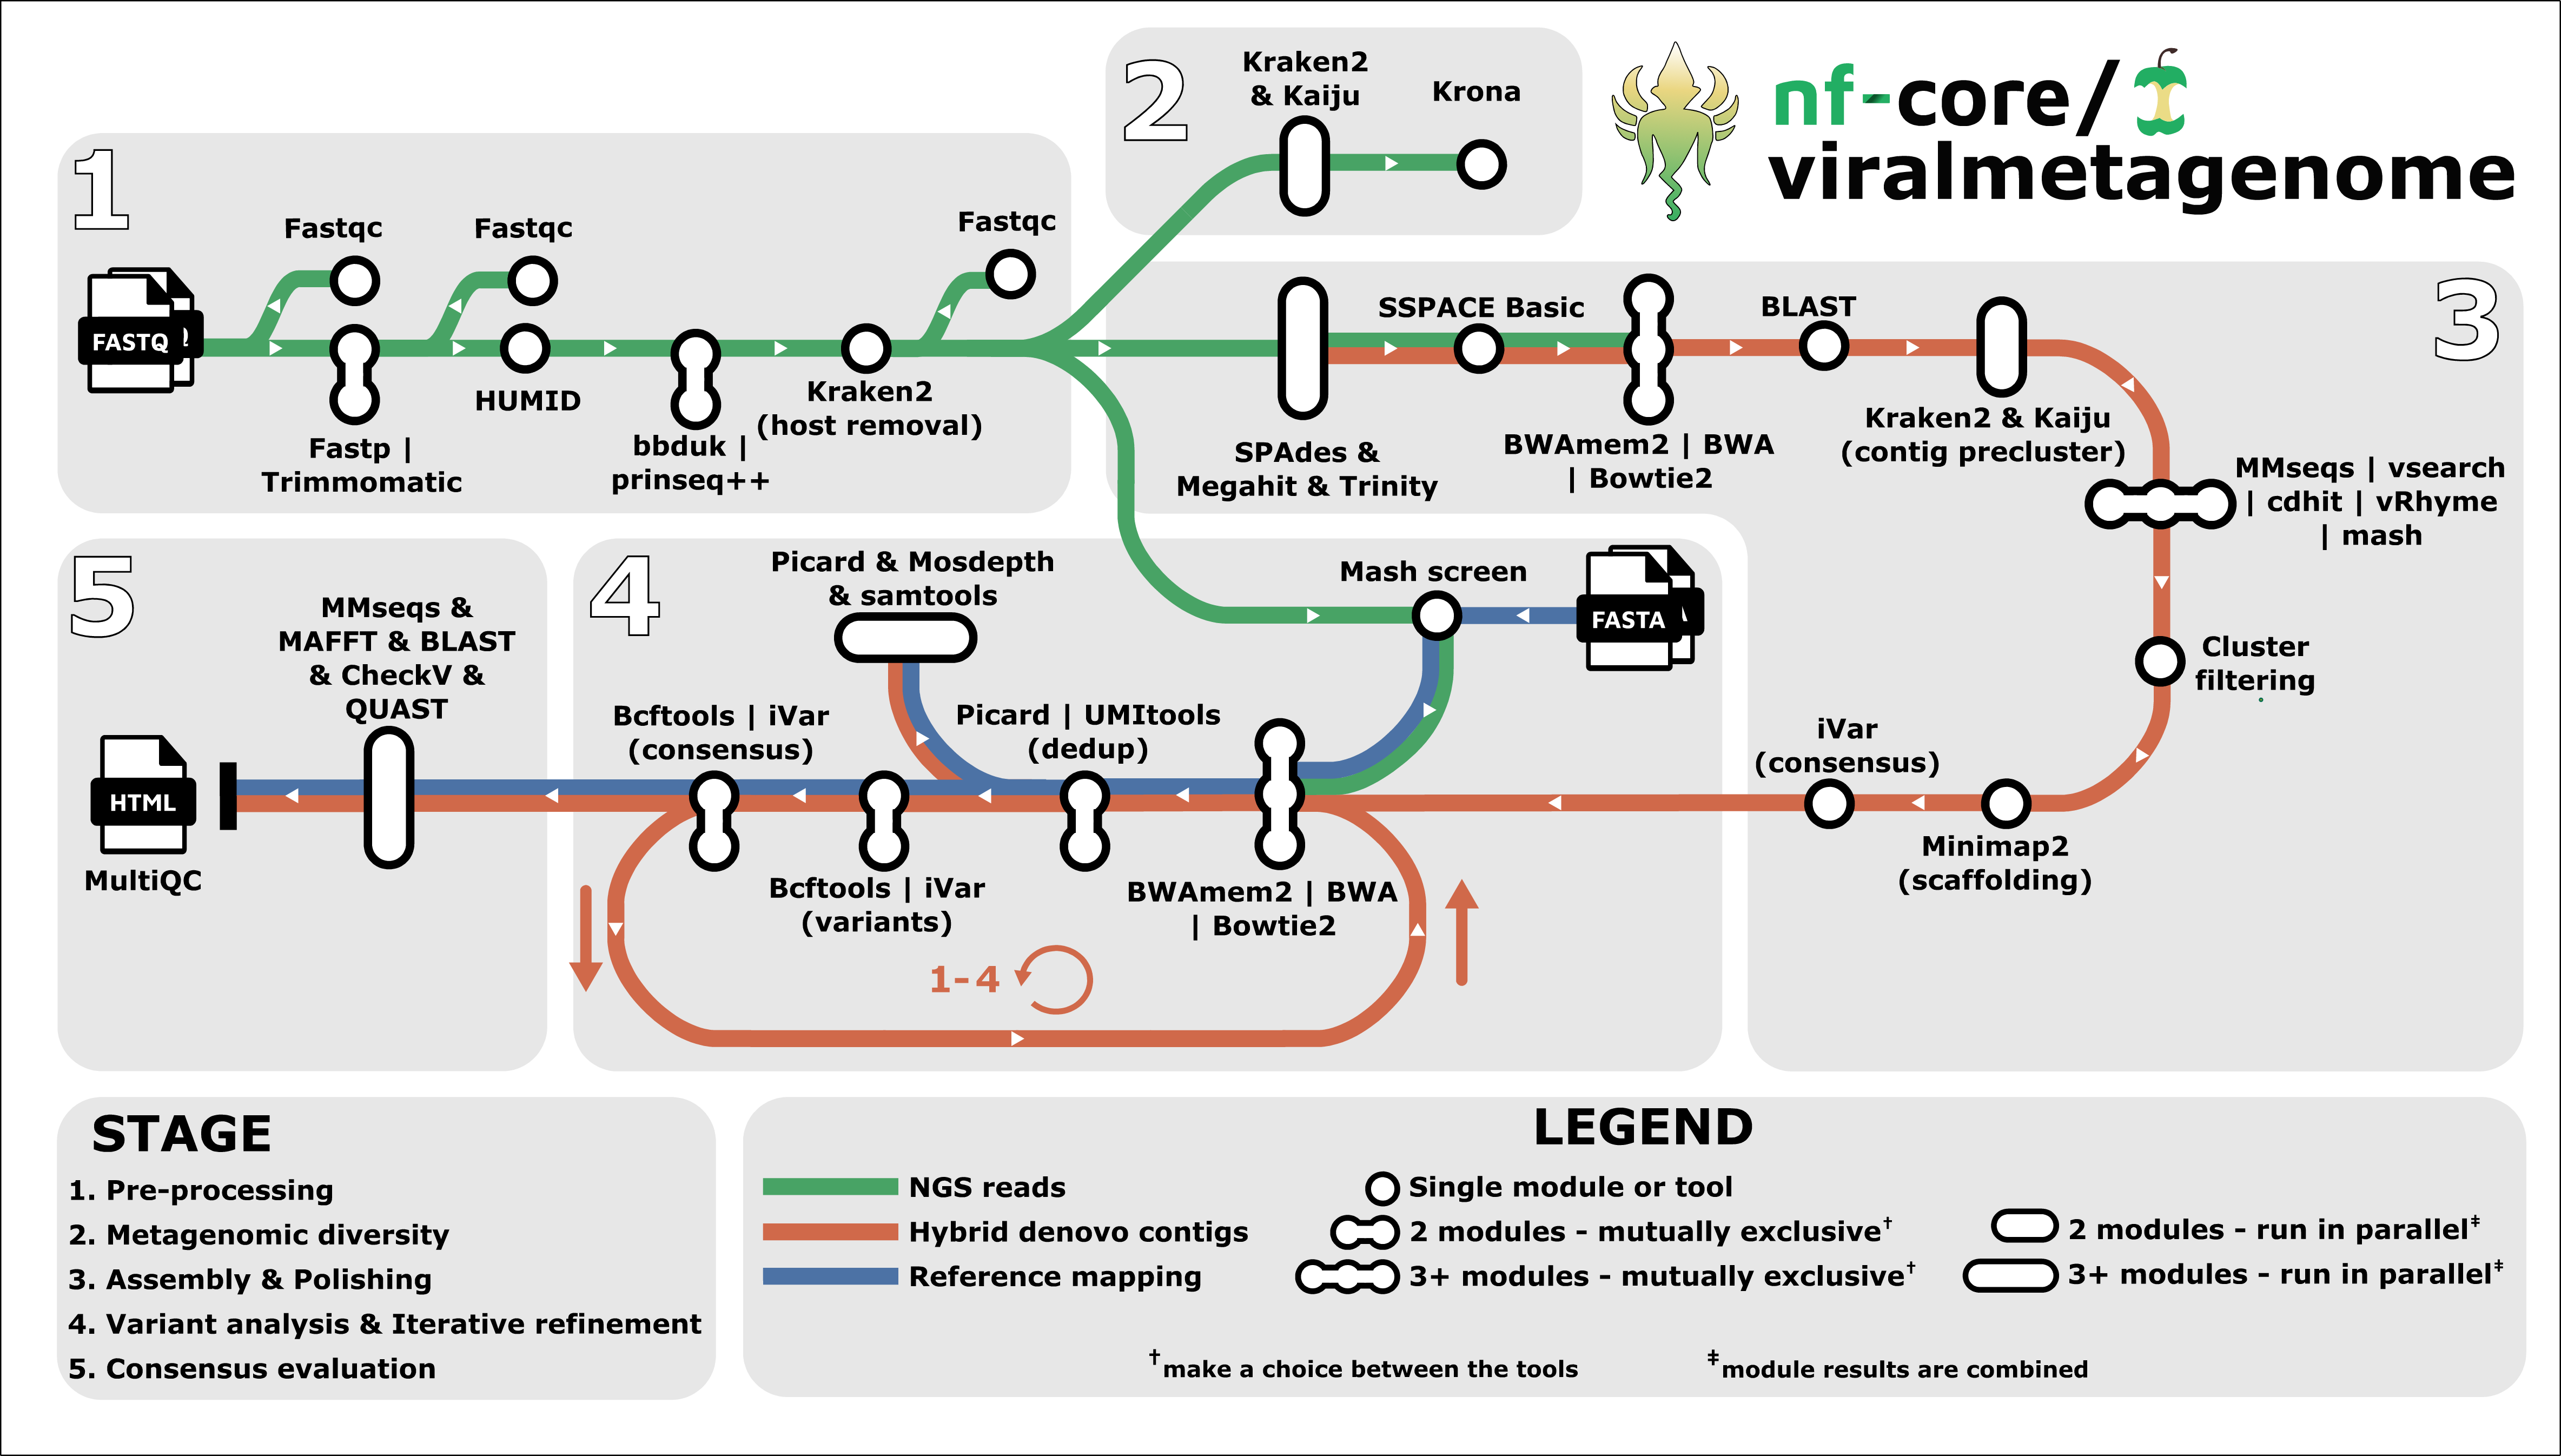
\includegraphics[width=1\textwidth]{Fig/fig1.png}
    \caption{Visual overview of the nf-core/viralmetagenome pipeline for untargeted viral genome reconstruction. nf-core/viralmetagenome processes short FASTQ files through optionally read preprocessing (adapter removal, quality filtering, host removal), metagenomic diversity assessment, de novo assembly with multiple assemblers, scaffolding with automated reference identification and contig taxonomy-guided clustering, and iterative consensus refinement through read mapping and variant calling. Quality control metrics, assembly statistics, and coverage data are integrated into interactive MultiQC reports and standardised overview tables for downstream analysis.}
    \label{fig:pipeline-workflow}
\end{figure*}

%% - Continue HERE %%
\section{Implementation}

Nf-core/viralmetagenome only requires nextflow and a container management system (Docker, Singularity, or Conda). The pipeline can be executed with this minimal setup:

\begin{verbatim}
nextflow run nf-core/viralmetagenome \
  -profile docker \
  --input samplesheet.csv \
  --output results
\end{verbatim}

Input data is provided through a sample sheet in CSV, TSV, YAML, or JSON format containing sample names and paths to FASTQ files. The pipeline supports both single-end and paired-end sequencing metagenomic data, and offers optional support for Unique Molecular Identifiers (UMIs) as well as optional merging of sequencing runs.

\subsection{Read preprocessing}

The read preprocessing module performs quality control and filtering of raw sequencing reads. Initial quality assessment is conducted using FastQC before and after each processing step to monitor data quality throughout the workflow. Adapter trimming and read processing are performed using either Fastp \cite{Chen2018-tu} (default) or Trimmomatic \cite{Bolger2014-si}. Fastp is overall faster and has automated adapter detection and trimming \cite{Chen2018-tu}. For libraries prepared with UMIs, deduplication is implemented using HUMID \cite{LarosUnknown-nx} and with UMI-tools \cite{Smith2017-nk} once reads are mapped to a reference. If sequencing run merging is required, this can be done after adapter trimming and read-level deduplication by specifying a group in the input samplesheet. Complexity filtering, implemented through BBduk \cite{BushnellUnknown-qy} or prinseq++ \cite{Cantu2019-vs}, removes low-complexity sequences containing repetitive elements that can lead to spurious alignments or misclassifications during downstream analysis. Host and contamination removal is performed using Kraken2 \cite{Wood2019-jl} against a user-specified host genome database. The default database contains a subset of the human genome. However, users are encouraged to employ more comprehensive databases, including complete host genome and transcriptome (human and otherwise), common sequencer contaminants, and bacterial genomes, to ensure thorough decontamination \cite{Forbes2025-mv}.

\subsection{Metagenomic diversity assessment}

Taxonomic classification of preprocessed reads is performed using two complementary approaches - Kaiju \cite{Menzel2016-tz} and Kraken2 \cite{Wood2019-jl} - to maximise detection sensitivity across diverse viral families. Results from both classifiers are visualised using Krona \cite{Ondov2011-yp}.

\subsection{\textit{De novo} assembly and clustering}

The assembly workflow implements a multi-assembler approach followed by clustering and scaffolding procedures. De novo assembly is performed using one or multiple assemblers: SPAdes \cite{Meleshko2021-gb} (configured for RNAviral mode by default), MEGAHIT \cite{Li2016-sd}, and Trinity \cite{Grabherr2011-ef}. This multi-assembler strategy capitalises on the distinct algorithmic strengths of each tool to maximise genome recovery across diverse viral families and variable read depths. Assembled contigs can be subjected to an optional extension step using SSPACE Basic \cite{Boetzer2011-dh}.

Reference identification is conducted through BLASTn \cite{Altschul1990-sy} searches against a comprehensive reference sequence pool, with the default being the latest clustered Reference Viral Database \cite{Goodacre2018-dw}. To facilitate identification of related genomic segments and appropriate reference sequences for contig scaffolding, the top five BLAST hits for each contig are retained and incorporated into the subsequent taxonomy-guided clustering step.

Taxonomy-guided clustering employs a two-stage process to cluster related contigs. Initial pre-clustering uses taxonomic assignments from both Kraken2 \cite{Wood2019-jl} and Kaiju \cite{Menzel2016-tz}. For more efficient targeted analyses, the user can opt to focus on specific taxonomic clades. Subsequent nucleotide similarity clustering is performed using one of six available algorithms: CD-HIT-EST \cite{Li2006-nj}, VSEARCH \cite{Rognes2016-ju}, MMseqs2 \cite{Steinegger2017-ci}, vRhyme \cite{Kieft2022-km}, or Mash \cite{Ondov2019-bo} with network-based community detection using the Leiden algorithm \cite{Traag2019-yd} or through single linkage.  All tools are valid options, though performance may vary depending on the dataset; for comprehensive benchmarking, we refer to Zielezinski et al. (2025) \cite{Zielezinski2025-vl} and Steinegger and Söding (2017) \cite{Steinegger2017-ci}.

As an optional filtering step of contig clusters, after assembly and extension, reads can be mapped to all contigs using BWAmem2 \cite{Vasimuddin2019-rb} (default), BWA \cite{Li2013-pp}, or Bowtie2 \cite{Langmead2019-wx}. Clusters are filtered based on the cumulated percentage of reads mapped to the contigs of a cluster. By filtering clusters, low-coverage assemblies can be identified that likely represent assembly artefacts.

The final scaffolding step maps all cluster members to the cluster representative using Minimap2 \cite{Li2018-gi}, followed by consensus calling with iVar \cite{Grubaugh2019-xd} to generate reference-assisted assemblies. Regions with zero coverage depth can optionally be represented by the reference genome to produce a more complete scaffold genome for consensus calling.

\subsection{Iterative consensus refinement and variant calling}

The consensus and variant calling module supports two distinct pathways: external reference-based analysis and scaffold refinement. In external reference-based analysis, users can provide reference genomes through the argument \texttt{--mapping\_constraints}, which allows specifying a separate reference genome or reference set for each sample. When multiple genomes are provided for a single sample, the genome with the highest similarity is used as a reference using Mash \cite{Ondov2019-bo}

Within the scaffold refinement, the pipeline can perform up to 4 cycles of iterative improvement (default 2) of the scaffolded de novo assembled contigs. Each iteration maps reads back to the current consensus using BWAmem2 \cite{Vasimuddin2019-rb}, BWA \cite{Li2013-pp}, or Bowtie2 \cite{Langmead2019-wx}, followed by variant calling and consensus generation with BCFtools \cite{Danecek2021-je} or iVar \cite{Grubaugh2019-xd}. Benchmarking by Bassano et al. \cite{Bassano2022-cl} showed that BCFtools outperformed iVar in precision and recall. iVar tends to detect more low-frequency variants, which may increase false positives but also reduce false negatives. Users are recommended to consider prioritising sensitivity or specificity when selecting the variant caller.

Optional deduplication can be performed using Picard or when UMI’s are available with UMI-tools \cite{Smith2017-nk}. Comprehensive mapping statistics are generated using samtools (flagstat, idxstats, stats) \cite{Danecek2021-je}, Picard CollectMultipleMetrics \cite{Broad-Institute2019-rv}, and coverage analysis with mosdepth \cite{Pedersen2018-mu}.

\subsection{Consensus Quality Control}

Comprehensive quality assessment of reconstructed viral genomes is performed through multiple complementary analyses. CheckV \cite{Nayfach2021-wl} estimates genome completeness and contamination. Consensus genomes undergo similarity analysis through BLASTn \cite{Altschul1990-sy} searches against the reference pool, and MMseqs \cite{Steinegger2017-ci} searches against comprehensive annotation databases such as Virosaurus \cite{Gleizes2020-rq}, enabling species identification, segment designation, host associations, and any other additional customised metadata embedded in the database.

Multiple sequence alignment using MAFFT \cite{Katoh2002-ox} aligns the final consensus genomes with the de novo contigs, the consensus genomes during iterations and the reference used for scaffolding, enabling assessment of assembly accuracy. Quality control metrics are integrated into interactive MultiQC reports \cite{Ewels2016-hs}, providing a comprehensive visualisation of the pipeline results. Standalone overview tables are generated by extracting key metrics from MultiQC into dataframes, facilitating downstream analysis of all samples.

\section{Applications}

To evaluate the performance of nf-core/viralmetagenome under challenging scenarios, we simulated coinfection scenarios by mixing paired-end reads from public HIV-1 genomes with varying diversity (80-99\% similarity), resulting in 13 samples (see supplementary table 2). Nf-core/viralmetagenome successfully identified coinfections in all mixed samples when genetic similarity was low to moderate ($\leq$ 96.7\% ANI). For highly similar mixtures (98.7\% ANI), the 2 original genomes were only identified and reconstructed once out of 3 times.
We determined the influence of the reference used during scaffolding on the final consensus genome. Here, we observed that the influence is small to negligible when the reference used closely matches ($\geq$ 96\%) the original genome. However, if the reference is more divergent, the number of mismatches between final consensus genomes could increase up to 187 nucleotides (Figure~\ref{fig:reference-influence}). This highlights the importance of appropriate reference selection for scaffolding or, in general, sequence alignment.

\begin{figure}[htbp]
    \centering
    \includegraphics[width=0.5\textwidth]{Fig/fig2.png}
    \caption{Boxplot of maximum observed differences between consensus sequences generated with different reference genomes during scaffolding. Mean highlighted by a diamond.}
    \label{fig:reference-influence}
\end{figure}

To validate nf-core/viralmetagenome's performance on real-world datasets, we applied the pipeline to publicly available metagenomic samples spanning viral pathogens for both humans and plants. Here, the pipeline successfully generated high-quality or near-complete genomes for all species across different viral families, including both segmented viruses (Lassa virus, Orthonairovirus, Tomato spotted wilt tospovirus) and non-segmented viruses (SARS-CoV-2, West Nile virus, Potato virus Y, Youcai mosaic virus,  and Monkeypox virus).

The computational requirements for analysing 28 samples of human viruses (supplementary methods) required 412 CPU hours and a maximum of 79GB RAM on an HPC system, excluding taxonomic classification steps. The automated reference-contig clustering strategy represents a considerable advancement over manual curation, reducing processing time while maintaining accuracy. However, this analysis also demonstrates that the pipeline's performance is influenced by the quality and comprehensiveness of reference databases, with closer reference similarity yielding more complete and accurate consensus genomes. This underscores the importance of maintaining up-to-date databases such as the Reference Viral Database \cite{Goodacre2018-dw} and Virosaurus \cite{Gleizes2020-rq}. The pipeline uses the Virosaurus-vertebrate database by default; users analysing plant pathogens should switch to the Virosaurus-plant database for optimal results. Since nf-core/viralmetagenome is primarily designed for eukaryotic viruses, bacteriophage analysis requires different approaches and users are encouraged to consider pipelines targeting phages such as VIRify \cite{Rangel-Pineros2022-wv}, VIBRANT \cite{Kieft2020-aq}, VirSorter2 \cite{Guo2021-rf}.


\section{Conclusion}

nf-core/viralmetagenome addresses a critical need in viral genomics by providing an automated, scalable solution for untargeted viral genome reconstruction. The pipeline successfully automates the traditionally time-consuming and manual execution process of viral genome assembly from metagenomic data through its integrated workflow of de novo contig assembly, automated reference selection, clustering algorithms, and iterative refinement strategies.

Our validation demonstrates the pipeline's broad applicability across diverse eukaryotic viral families, achieving high-quality genome reconstruction while ensuring reproducibility and ease of deployment across different computational environments.

As viral surveillance and outbreak response increasingly rely on metagenomic sequencing, automated pipelines like viralmetagenome will be essential for the timely identification of pathogen strains. The pipeline represents a significant step forward in making viral genome reconstruction accessible to researchers without requiring extensive bioinformatics expertise, facilitating broader adoption of metagenomic approaches in viral research and public health applications.


\section*{Acknowledgments}
 J.K, P.L. and L.K  acknowledges support from the Research Foundation - Flanders (Fonds voor Wetenschappelijk Onderzoek – Vlaanderen, G005323N and G051322N, 1SH2V24N, 12X9222N).

\section*{Author Contributions}
J.K. designed and implemented the pipeline, performed validation analyses, and wrote the manuscript. P.L. and L.K. supervised the project and provided critical feedback. All authors reviewed and approved the final manuscript.

\section*{Data Availability}
The nf-core/viralmetagenome pipeline is freely available at https://github.com/nf-core/viralmetagenome.
The raw data and analysis code is available on https://github.com/Joon-Klaps/nf-core-viralmetagenome-manuscript/.

\section*{Conflict of Interest}
The authors declare no competing interests.

